%%=============================================================================
%% Methodologie
%%=============================================================================

\chapter{\IfLanguageName{dutch}{Methodologie}{Methodology}}%
\label{ch:methodologie}

Deze bachelorproef onderzoekt en verbetert de API-kwaliteit bij BrightAnalytics door de iteratieve ontwikkeling van de BrightEats API. Onderzoek en ontwikkeling gaan hand in hand. De inzichten uit het onderzoek worden direct toegepast op de API, en de ervaringen tijdens de ontwikkeling sturen het onderzoek bij.

Ik ga ervan uit dat ik elke week minstens \'e\'en dag kan werken aan de bachelorproef. De deadlines zijn echter flexibel, aangezien de API-ontwikkeling continu doorloopt en de planning kan be\"invloeden.

Na evaluatie in de literatuurstudie blijkt implementatie van HATEOAS niet geschikt voor de BrightEats API. In plaats daarvan focussen we op het opstellen van een interne guide, gebaseerd op best practices en vergelijkbaar met de Zalando RESTful API and Event Scheme Guidelines. Daarnaast wordt een uitgebreide OpenAPI-specificatie voor de API ontwikkeld.

\section{Fase 1: Onderzoek en eerste opzet API}

\textbf{Deadline: 17 november 2024}

Deze fase is gericht op het verzamelen van kennis over kwalitatieve API-ontwikkeling en het defini\"eren van een eerste set best practices voor BrightEats. Ik bestudeer de principes van REST, HATEOAS en OpenAPI en hun belang voor API-kwaliteit en formuleer concrete aanbevelingen voor de BrightEats API.

\bigskip

\textbf{We zoeken een antwoord op de volgende vragen:}
\begin{itemize}
  \item Wat zijn de principes van REST?
  \item Hoe dragen deze bij aan betere API's?
  \item Welke best practices zijn er voor URI-structuur, HTTP-methoden, response codes en versiebeheer?
  \item Hoe houden we onze Laravel-API RESTful?
  \item Wat zijn de principes en voordelen van HATEOAS?
  \item Hoe kunnen we HATEOAS implementeren in een Laravel-API?
  \item Hoe maken we optimaal gebruik van HATEOAS in de frontend van BrightEats?
  \item Wat is OpenAPI en hoe kan dit worden toegepast in de documentatie van een Laravel-API?
\end{itemize}

\textbf{Deliverables:}

\begin{itemize}
  \item Literatuurstudie over REST, HATEOAS en OpenAPI.
  \item Best practices voor de implementatie in de BrightEats API en frontend.
\end{itemize}

\section{Fase 2: Iteratieve ontwikkeling en verfijning BrightEats API}

\textbf{Deadline: 8 december 2024}

\bigskip
Gedurende deze fase refactor ik de BrightEats API iteratief naar een RESTful design, terwijl we ook de OpenAPI-specificatie definiëren. We doen dit stap per stap, zonder de hele API in één keer te herschrijven. De focus ligt op het toepassen van de best practices die we in fase 1 hebben geformuleerd.

\subsection{Ontwikkeling van de API (doorlopend)}

\bigskip
Elke week doorloop ik de volgende stappen:

\begin{enumerate}
  \item \textbf{Plannen:} Ik bepaal welke functionaliteiten ik aan de API zal toevoegen (of welke code ik ga refactoren om zo aan de nieuwe best practices te voldoen)
  \item \textbf{Ontwerpen:} Ik ontwerp de nieuwe/gerefactorde functionaliteiten met de best practices in gedachten.
  \item \textbf{Implementeren:} Ik programeer de nieuwe/gerefactorde functionaliteiten in de API.
  \item \textbf{Testen:} Ik test de nieuwe/gerefactorde functionaliteiten grondig.
  \item \textbf{Evalueren:} Ik beoordeel de kwaliteit, structuur en gebruikte best practices.
  \item \textbf{Best practices bijstellen:} Ik pas de richtlijnen aan op basis van de evaluatie en feedback.
\end{enumerate}

\textbf{Deliverables:}

\begin{itemize}
  \item Wekelijkse updates van de BrightEats API.
  \item Documentatie van de API met OpenAPI specificaties.
  \item Logboek met gemaakte keuzes en evaluaties.
\end{itemize}

\section{Fase 3: Synthese, aanbevelingen en afronding}

\textbf{Deadline: 15 december 2025}

\bigskip
In de laatste fase vat ik mijn bevindingen samen en formuleer ik een antwoord op de onderzoeksvraag. Wat was de exacte kost van het implementeren van OpenAPI en RESTfulness in de BrightEats API? Welke voordelen en nadelen bracht dit met zich mee? Welke best practices kunnen we formuleren voor de ontwikkeling van API's bij BrightAnalytics?

\subsection{Synthese \& Aanbevelingen}

\textbf{Deadline: 15 januari 2025}

\bigskip
Ik schrijf de conclusie en aanbevelingen voor BrightAnalytics. Hierbij beantwoord ik de deelvragen en onderzoeksvraag en formuleer ik concrete best practices voor de ontwikkeling van RESTful API's bij BrightAnalytics.

\subsection{Afronding bachelorproef}

\textbf{Deadline: 10 januari 2025}

\bigskip
Ik werk de bachelorproef af, rekening houdend met de feedback van de promotor en de lead developer bij BrightAnalytics.

\textbf{Deliverables:}

\begin{itemize}
  \item Concrete aanbevelingen voor beter API-ontwerp.
  \item Finale versie van de bachelorproef.
\end{itemize}

\section{Gantt chart}

\begin{figure}[H]
  \centering
  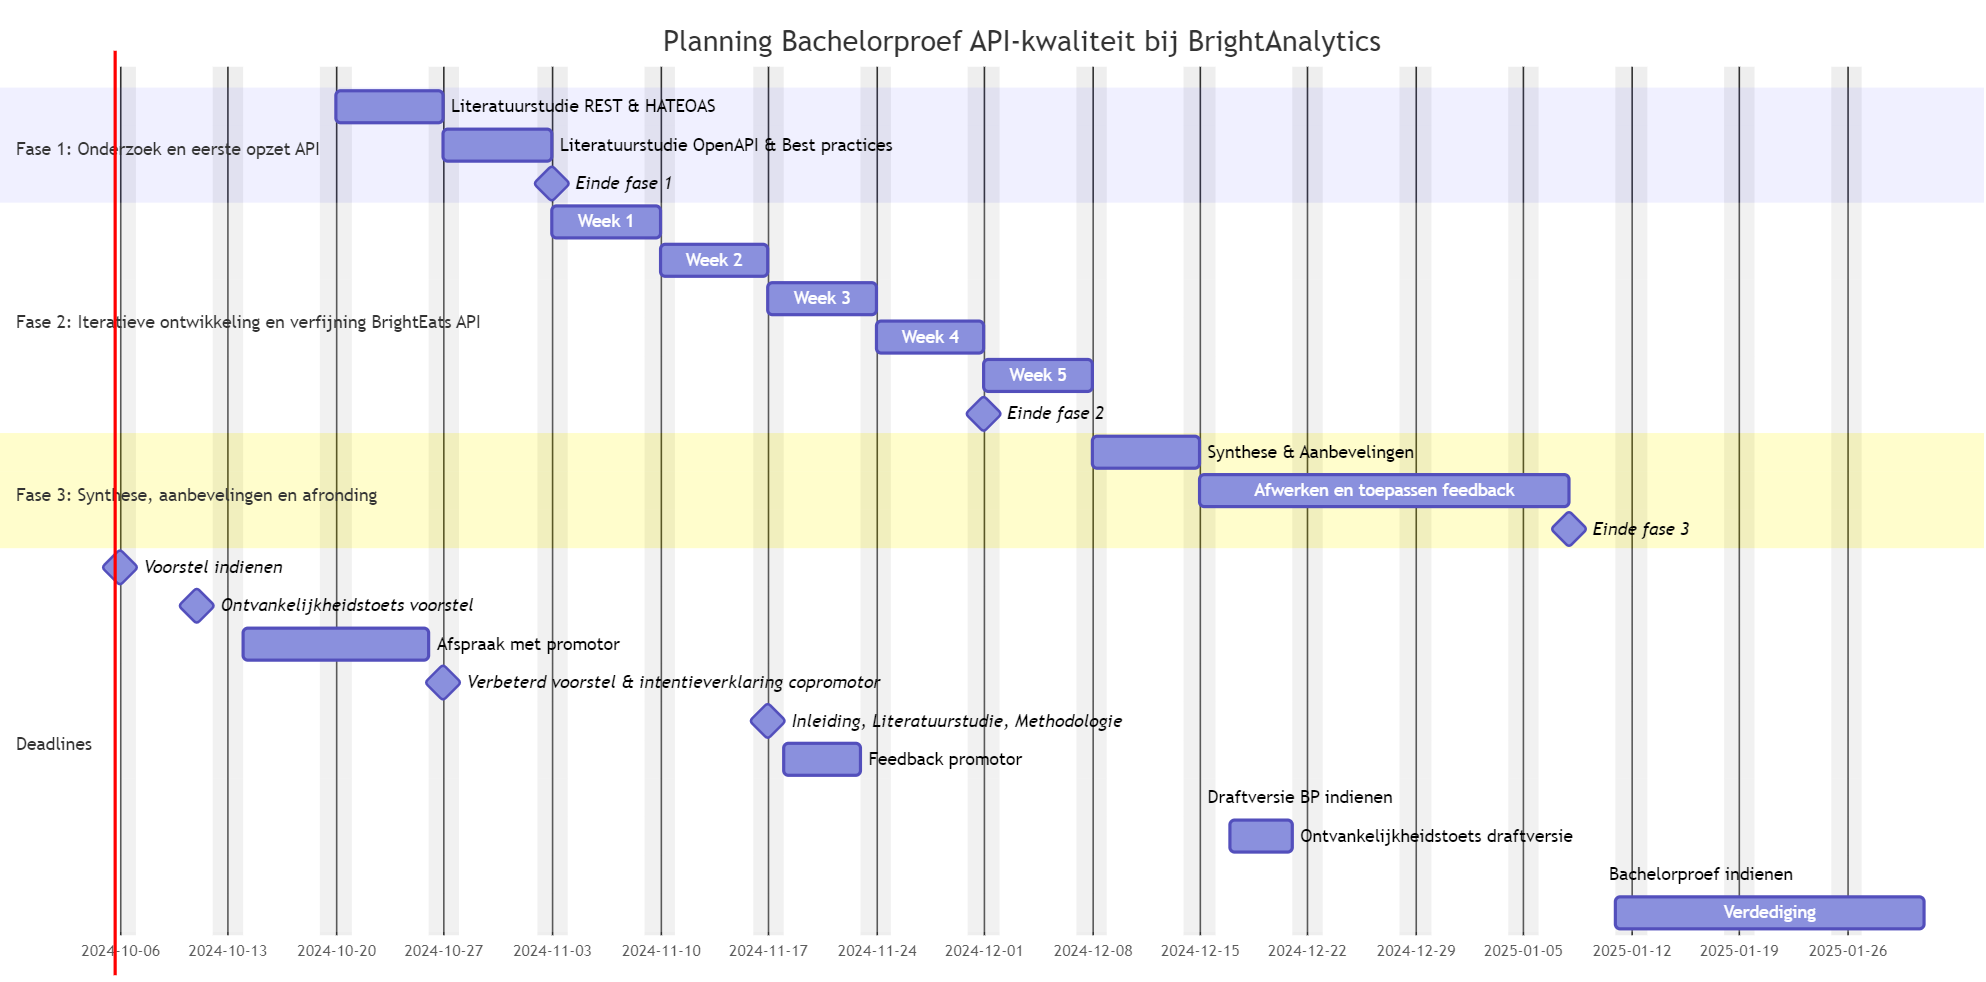
\includegraphics[width=0.8\textwidth]{gantt.png}
  \caption{Gantt chart van de methodologie}
  \label{fig:gantt}
\end{figure}
